\documentclass{bredelebeamer}

%%%%%%%%%%%%%%%%%%%%%%%%%%%%%%%%%%%%%%%%%%%%%%%%

\title[Programación en MatLAB]{Introducción a la programación con MatLAB}
\subtitle{Módulo 06 - Funciones definidas por el usuario}

\author{Autor1 - Autor2 - Autor3\inst{1}}
\institute[UTN.BA]
{
  \inst{1}%
  Universidad Tecnológica Nacional\\
  Facultad Regional Buenos Aires
  }

\date{dia mes 2018}

\subject{Taller de programación}

\logo{

\includegraphics[scale=0.15]{images/logo.png}
}

%%%%%%%%%%%%%%%%%%%%%%%%%%%%%%%%%%%%%%%%%%%%%%%%%%%%%%%%%%%%%%%%%%%%%
\begin{document}

\begin{frame}
  \titlepage 
\end{frame}


%%%%%%%%%%%%%%%%%%%%%%%%%%%%%%%%%%%%%%%%%%%%%%%%%%%%%%%%%%%%%%%%%%%%%

% Funciones definidas por el usuario

%%%%%%%%%%%%%%%%%%%%%%%%%%%%%%%%%%%%%%%%%%%%%%%%%%%%%%%%%%%%%%%%%%%%%
\section{Funciones definidas por el usuario}

\begin{frame}{Introducción}
\begin{center}
MATLAB permite definir funciones propias. Las funciones definidas por el usuario se almacenan como archivos .m y matlab puede acceder a ellas si están almacenadas en el directorio de trabajo actual.
\end{center}
Hasta ahora, por ejemplo la función interna: $cos(x)$
\begin{itemize}
\item La función se llama cos
\item Toma la entrada del usuario dentro de paréntesis (en este caso x)
\item Calcula un resultado\\
\end{itemize}
\begin{block}{Tener en cuenta}
Las funciones definidas por el usuario funcionan del mismo modo.
\end{block}
\end{frame}

\begin{frame}{Funciones definidas por el usuario}
\begin{itemize}
\item Las funciones definidas por el usuario se crean en archivos .m
\item Cada una debe comenzar con una línea de definición de función que contenga
\begin{itemize}
\item la palabra reservada \textbf{function}
\item Una variable que defina la salida de función
\item Un nombre de función
\item Una variable que se use para el argumento de entrada
\end{itemize}
\end{itemize}
Sintaxis:
\begin{center}
\textbf{function output = my\_function(variable)}
\end{center}
Donde:
\begin{itemize}
\item Argumento de entrada: variable
\item Nombre de la función: my\_function
\item Argumento de salida: output
\end{itemize}
\end{frame}

\begin{frame}{Funciones definidas por el usuario}
Se deben tener en cuenta las siguientes consideraciones:
\begin{itemize}
\item El nombre del archivo .m debe ser el mismo que el nombre de la función.
\item El nombre de la función debe comenzar con una letra.
\item El nombre de la función puede formarse con letras, números y guión bajo.
\item No se pueden usar nombres reservados.
\item Permite cualquier longitud.
\end{itemize}
\end{frame}

\begin{frame}{Ejercicio práctico xx}
\begin{center}
Realice una función que convierte minutos en segundos.
\end{center}
\end{frame}

\begin{frame}{Funciones con entradas y salidas múltiples}
Las funciones definidas por el usuario pueden requerir múltiples entradas y múltiples salidas. La sintaxis es:\\
\begin{center}
\textbf{function [output\_1 output\_2] = my\_function(variable\_1, variable\_2)}
\end{center}
Siendo la forma de invocar a la función:
\begin{center}
\textbf{[output\_1 output\_2] = my\_function(variable\_1, variable\_2)}
\end{center}
\end{frame}

\begin{frame}{Ejercicio práctico xx}
\begin{enumerate}
\item Escribir una función para multiplicar dos vectores punto a punto.
\item Escribir una función que dado un valor de tiempo calcule la distancia, velocidad y aceleración de un automóvil teniendo en cuenta:
\begin{itemize}
\item aceleracion = 0.5*t
\item velocidad = aceleracion*t
\item posición = vel *t
\end{itemize}
\end{enumerate}
\end{frame}

\begin{frame}{Funciones sin entrada o salida}
Las funciones definidas por el usuario pueden no requerir de entradas y salidas. La sintaxis es:\\
\begin{center}
\textbf{function [] = my\_function()}
\end{center}
Siendo la forma de invocar a la función:
\begin{center}
\textbf{[] = my\_function()}
\end{center}
\end{frame}

\begin{frame}{Variables locales y globales}
\begin{itemize}
\item \textbf{Variables locales:} Son las variables definidas dentro de una función. Estas existen sólo para el uso de la función, no se almacenan en el área de trabajo (workspace). Las funciones deben estar completamente autocontenidas.
\item \textbf{Variables globales:} Están disponibles para todas las partes de un programa de cómputo. Se definen mediante el comando \textbf{global} variable.
\end{itemize}
\begin{block}{Tener en cuenta}
Funciones autocontenido: Sólo pueden obtener información de su programa a través de los argumentos de entrada y la única forma en que pueden entregar información es a través de la salida de la función.
\end{block}
\begin{alertblock}{Importante}
No es una buena práctica de programación utilizar variables globales.
\end{alertblock}
\end{frame}

%%%%%%%%%%%%%%%%%%%%%%%%%%%%%%%%%%%%%%%%%%%%%%%%%%%%%%%%%%%%%%%%%%%%%

% Sección de consultas

%%%%%%%%%%%%%%%%%%%%%%%%%%%%%%%%%%%%%%%%%%%%%%%%%%%%%%%%%%%%%%%%%%%%%

\section{Consultas}
\begin{frame}{Consultas}
\begin{center}

\includegraphics[scale=0.3]{images/consultas.png}
\end{center}
\end{frame}


%%%%%%%%%%%%%%%%%%%%%%%%%%%%%%%%%%%%%%%%%%%%%%%%%%%%%%%%%%%%%%%%%%%%%

% Sección de bibliografía

%%%%%%%%%%%%%%%%%%%%%%%%%%%%%%%%%%%%%%%%%%%%%%%%%%%%%%%%%%%%%%%%%%%%%

\section{Bibliografia}

\begin{frame}{Bibliografía}
\begin{columns}
\begin{column}{0.5\textwidth}
\begin{center}

\includegraphics[scale=0.4]{images/biblio1.png}
\end{center}
\end{column}
\begin{column}{0.5\textwidth}
\begin{center}
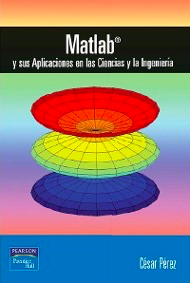
\includegraphics[scale=0.5]{images/biblio2.png}
\end{center}
\end{column}
\end{columns}
\end{frame}

\end{document}
